\documentclass{article}
\usepackage{amsmath}
\usepackage{amssymb}
\usepackage[a4paper, top=25mm, bottom=25mm, left=25mm, right=25mm]{geometry}
\usepackage{pgfplots}
\pgfplotsset{compat=1.18}
\usepackage{mathtools}
\usepgfplotslibrary{polar}
\usepgfplotslibrary{fillbetween}
\usepackage{tikz}
\usetikzlibrary{arrows.meta}

\begin{document}
\pagestyle{empty}
\large

\begin{center}
2019-2020 Summer \\MAT124 Final\\(28/08/2020)
\end{center}

\noindent 1. Find the maximum and minimum values of the function $f(x,y)=x^2+y^2-3y$ on the closed disk $x^2+y^2\leq4$.

\hfill

\noindent 2. The velocity of a particle moving in space is

\begin{equation*}
\mathbf{V}(t)=\ln t\,\mathbf{i} +\sin t\,\mathbf{j}+ t^3\,\mathbf{k}
\end{equation*}

\hfill

\noindent Find the particle's position as a function of $t$ if the position at time $t=1$ is $\mathbf{R}(1)=2\mathbf{i}+\mathbf{j}-\mathbf{k}$.

\hfill

\noindent 3. Evaluate the integral $\displaystyle \int_0^1\int_{y^2}^1 y^3\cos x^3\,dx\,dy$.

\hfill

\noindent 4. Let $R$ be the region lying inside $r=1$ and outside $r=1+\cos\theta$.

\hfill

(i) Sketch the graph of the region $R$.

\hfill

(ii) Set up (but do not evaluate) a double integral in polar coordinates for the area of the region $R$.

\hfill

\noindent 5. Let $S$ be the surface of the portion of the cone $z^2=x^2+y^2$ that is contained in the cylinder $x^2+y^2=9$.

\hfill

(i) Sketch the graph of $S$.

\hfill

(ii) Evaluate the surface area using polar coordinates.

\hfill

\noindent 6. Let $S$ be the region bounded by the paraboloids $z=8-x^2-y^2$ and $z=x^2+y^2$.

\hfill

(i) Using the spherical coordinates, set up (but do not evaluate) an integral for the volume of the solid $S$.

\hfill

(ii) Using the cylindrical coordinates, set up (but do not evaluate) an integral for the volume of the solid $S$.

\newpage

\begin{center}
2019-2020 Summer Final (28/08/2020) Solutions\\
(Last update: 8/5/25 (5th of August) 1:53 AM)
\end{center}

\noindent 1) Determine the critical points by setting $f_x=f_y=0$.

\[f_x=2x,\quad f_y=2y-3\]
\[f_x=f_y=0\implies x=0,\quad y=\frac32\]

\noindent The \textit{only} critical point occurs at $(0,3/2)$. The value of the function at this point is $f(0, 3/2) = 0^2 + (3/2)^2 -3(3/2)=-9/4$.

\hfill

\noindent Using Lagrange multipliers, find the corresponding points on the boundary. Let $g(x,y)=x^2+y^2-4$ be the constraint. Solve the system of equations below.

\[
\left.
\begin{array}{ll}
\displaystyle\nabla f =\lambda \nabla g\\
\displaystyle g(x,y) = 0
\end{array}
\right\}\quad
\nabla f = \left\langle2x,2y-3\right\rangle=\lambda\left\langle2x,2y\right\rangle= \lambda\nabla g
\]

\[2x(1-\lambda)=0\implies x=0\quad\text{or}\quad\lambda=1\]
\[2y(1-\lambda)-3=0\implies1-\lambda=\frac3{2y}\implies\lambda=1-\frac3{2y}\]

\[x=0\implies g(0,y)=0^2+y^2-4=0\implies y=\pm2\]
\[\lambda=1\implies 2y-3=2y\implies 0\neq-3\quad\therefore\lambda\neq-1\]

\hfill

\noindent Evaluate $f$ at the points $(0,2)$ and $(0,-2)$.

\[f(0,2)=0^2+2^2-3\cdot2=-2,\quad f(0,-2)=0^2+(-2)^2-3\cdot(-2)=10\]

\hfill

\noindent Compare the values $f(0,3/2),\:f(0,2),\:f(0,-2)$.

\[\boxed{f_{\text{max}}=f(0,-2)=10,\quad f_{\text{min}}=f(0,3/2)=-9/4}\]

\hfill

\noindent 2) The velocity of a particle can be obtained by taking the first derivative of the position vector of the particle. Since we have the velocity of the particle, we can take the antiderivative. The velocity vector is defined for $t>0$. It is continuous and integrable for $t>0$.

\[\mathbf{V}(t)=\ln t\,\mathbf{i}+\sin t\,\mathbf{j}+t^3\,\mathbf{k}\]

\[\int\mathbf{V}(t)\,dt=\left(\int\ln t\,dt\right)\,\mathbf{i}+\left(\int\sin t\,dt\right)\,\mathbf{j}+\left(\int t^3\,dt\right)\,\mathbf{k}\]

\hfill

\noindent The first integral on the right side can be evaluated with integration by parts. The second integral is related to the integration of trigonometric functions. The last integral is just ordinary integration. The position vector is as follows.

\[\mathbf{R}(t)=(t\ln t- t+c_1)\,\mathbf{i}+(-\cos t+c_2)\,\mathbf{j}+\left(\frac{t^4}4+c_3\right)\,\mathbf{k}\]

\newpage

\noindent Evaluate $\mathbf{R}(1)$ to find the constants.

\[\mathbf{R}(1)=(-1+c_1)\,\mathbf{i}+(-\cos1+c_2)\,\mathbf{j}\,+\left(\frac14+c_3\right)\,\mathbf{k}=2\mathbf{i}+\mathbf{j}-\mathbf{k}\]

\[c_1=3,\quad c_2=1+\cos1,\quad c_3=-\frac54\]

\hfill

\noindent Rewrite the position vector by substituting the numbers into the constants.

\[\boxed{\mathbf{R}(t)=(t\ln t-t+3)\,\mathbf{i}+(-\cos t + 1 + \cos 1)\,\mathbf{j}+\left(\frac{t^4}4-\frac54\right)\,\mathbf{k}}\]

\hfill

\noindent 3) It is difficult to solve the integral with this order of integration. Sketch the region and change the order of integration.

\begin{center}
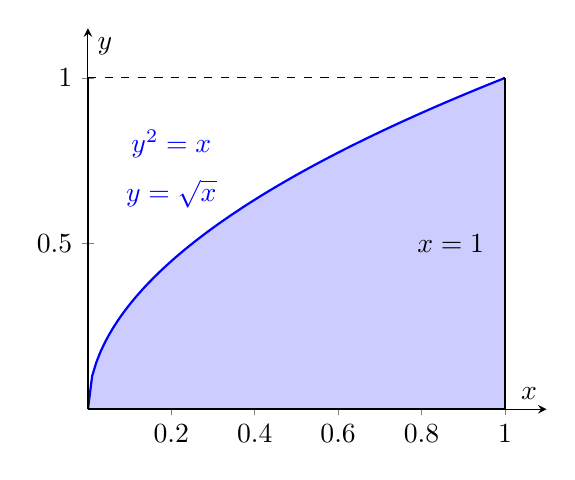
\begin{tikzpicture}
  \begin{axis}[
      axis lines = middle,
      xlabel = $x$, ylabel = $y$,
      domain=0:1,
      ymin=0, ymax=1.15,
      xmin=0, xmax=1.1,
      samples=100,
      clip=true,
      scale=0.85
    ]
    
    \addplot [
      name path=A,
      domain=0:1,
      draw=none,
    ] {sqrt(x)};

    \path[name path=B] (axis cs:0,1) -- (axis cs:1,1);
    \path[name path=C] (axis cs:0,0) -- (axis cs:0,1);
    \path[name path=D] (axis cs:0,0) -- (axis cs:1,0);

    \addplot [fill=blue!20, draw=none] fill between [of=D and A, soft clip={domain=0:1}];
    
    \addplot[blue, thick] {sqrt(x)};
    \addplot[thick] coordinates {(0,0) (0,1)};
    \addplot[thick] coordinates {(1,0) (1,1)};
    \addplot[thick] coordinates {(0,0) (1,0)};
    \draw[dashed] (axis cs: 0,1) -- (axis cs: 1,1);
    \node at (axis cs: 0.87, 0.5) {$x=1$};
    \node[blue] at (axis cs: 0.2, 0.8) {$y^2=x$};
    \node[blue] at (axis cs: 0.2, 0.65) {$y=\sqrt{x}$};

  \end{axis}
\end{tikzpicture}
\end{center}
\begin{align*}
\int_0^1\int_{y^2}^1y^3\cos\left(x^3\right)\,dx\,dy&=\int_0^1\int_0^{\sqrt x}y^3\cos\left(x^3\right)\,dy\,dx=\int_0^1\cos\left(x^3\right)\left[\frac{y^4}4\right]_{y=0}^{y=\sqrt x}\,dx\\\\&=\frac14\int_0^1x^2\cos\left(x^3\right)\,dx=\frac1{12}\bigg[\sin\left(x^3\right)\bigg]_0^1=\boxed{\frac1{12}\sin1}\end{align*}

\hfill

\noindent 4)


\hfill

\begin{minipage}{0.5\textwidth}

(i)

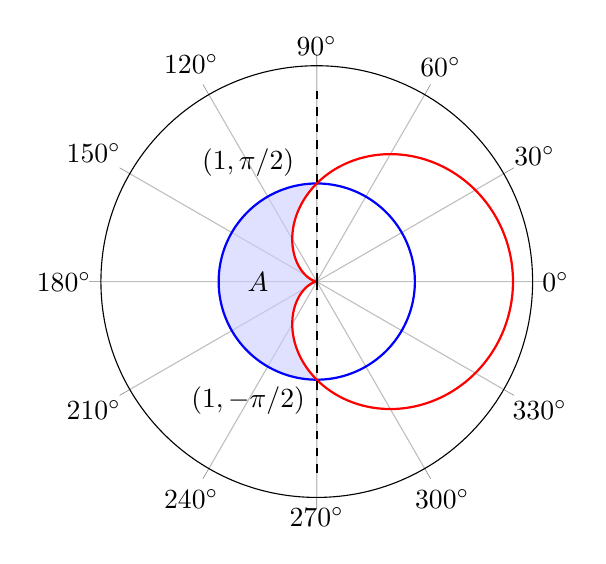
\begin{tikzpicture}
  \begin{polaraxis}[ytick=\empty, axis y line=none, scale=0.8, xticklabel=$\pgfmathprintnumber{\tick}^\circ$,]
    \addplot [
      domain=pi/2:3*pi/2,
      samples=300,
      draw=none,
      name path=A,
      data cs=polarrad,
    ] {1};

    \addplot [
      domain=pi/2:3*pi/2,
      samples=300,
      draw=none,
      name path=B,
      data cs=polarrad,
    ] {1+cos(deg(x))};

    \addplot [
      blue!20,
      fill opacity=0.6,
    ] fill between[of=A and B];

    \addplot [
      domain=0:2*pi,
      samples=300,
      thick,
      blue,
      data cs=polarrad,
    ] {1};

    \addplot [
      domain=0:2*pi,
      samples=300,
      thick,
      red,
      data cs=polarrad,
    ] {1+cos(deg(x))};

    \draw[black, thick, dashed] (axis cs: 90,0) -- (axis cs: 90,2);
    \draw[black, thick, dashed] (axis cs: -90,0) -- (axis cs: -90,2);

    \node at (axis cs:120,1.4) {$(1,\pi/2)$};
    \node at (axis cs:-120,1.4) {$(1,-\pi/2)$};
    \node at (0,-0.6) {$A$};

  \end{polaraxis}
\end{tikzpicture}
\end{minipage}
\begin{minipage}{0.4\textwidth}
\begin{equation*}
\text{(ii)}\quad\boxed{A=\int_{\pi/2}^{3\pi/2}\int_{1+\cos\theta}^1r\,dr\,d\theta}
\end{equation*}
\end{minipage}

\newpage

\noindent 5.

\hfill

\noindent (i)
\begin{center}
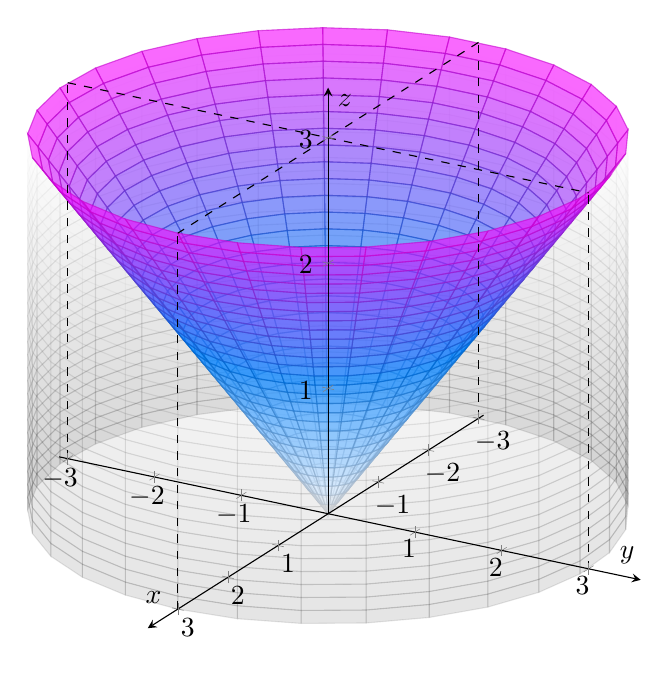
\begin{tikzpicture}
  \begin{axis}[
    view={120}{30},
    axis on top,
    axis lines=center,
    xlabel={$x$},
    ylabel={$y$},
    zlabel={$z$},
    xtick={-3,-2,-1,1,2,3},
    ytick={-3,-2,-1,1,2,3},
    xmin=-3.1, xmax=3.6,
    ymin=-3.1, ymax=3.6,
    zmin=0, zmax=3.4,
    samples=30,
    domain=0:360,
    y domain=0:3,
    scale=1.7,
  ]
  
\addplot3[surf, colormap/blackwhite, shader=flat, opacity=0.1] ({3*cos(x)}, {3*sin(x)}, {y});
\addplot3[surf, colormap/cool, z buffer=sort, opacity=0.6] ({y*cos(x)}, {y*sin(x)}, {y});

\draw[dashed] (axis cs:0,-3,3) -- (axis cs:0,3,3);
\draw[dashed] (axis cs:-3,0,3) -- (axis cs:3,0,3);

\draw[dashed] (axis cs:-3,0,0) -- (axis cs:-3,0,3);
\draw[dashed] (axis cs:0,3,0) -- (axis cs:0,3,3);
\draw[dashed] (axis cs:3,0,0) -- (axis cs:3,0,3);
\draw[dashed] (axis cs:0,-3,0) -- (axis cs:0,-3,3);

\end{axis}
\end{tikzpicture}
\end{center}
\begin{align*}
A&=\iint_D\sqrt{1+\left(\frac{\partial z}{\partial x}\right)^2 +\left(\frac{\partial z}{\partial y}\right)^2}\,dA= \iint_D\sqrt{1+\left(\frac{x}{\sqrt{x^2+y^2}}\right)^2 +\left(\frac{y}{\sqrt{x^2+y^2}}\right)^2}\,dA \\\\&=\iint_D\sqrt{1+\left(\frac{x^2+y^2}{x^2+y^2}\right)}\,dA=\iint_D\sqrt{1+1}\,dA=\sqrt{2}\iint_D\,dA
\end{align*}

\hfill

\noindent If we switch to polar coordinates, we can easily evaluate the integral.

\begin{equation*}A=\sqrt2\int_0^{2\pi}\int_0^3\,r\,dr\,d\theta=\sqrt2\int_0^{2\pi}\left[\frac{r^2}2\right]_{r=0}^{r=3}\,d\theta=\sqrt2\int_0^{2\pi}\frac92\,d\theta=\boxed{9\pi\sqrt2}\end{equation*}

\hfill

\noindent 6)

\hfill

\noindent (i) For spherical coordinates, we have

\[
\begin{array}{c}
z=\rho\cos\phi\\
r=\rho\sin\phi\\
x^2+y^2+z^2=\rho^2\\
dV=\rho^2\sin\phi\,d\rho\,d\phi\,d\theta
\end{array}\quad\rightarrow\quad
\begin{array}{lc}
z=8-x^2-y^2\implies\rho\cos\phi=8-\rho^2\sin^2\phi & (1)\\[0.2cm]
z=x^2+y^2\implies\rho\cos\phi=\rho^2\sin^2\phi & (2)\\
\end{array}
\]

\hfill

\noindent Now, notice that we have two distinct upper bounds for $\rho$. From $\phi=0$ to the angle of intersection, the integration is bounded above by $z=8-x^2-y^2$, where from the angle of intersection to $\phi=\pi/2$, the integration is bounded above by $z=x^2+y^2$.

\hfill

\noindent Solve $(1)$ for $\rho$ to find the upper bound.

\[\rho\cos\phi=8-\rho^2\sin^2\phi\implies\rho^2\sin^2\phi+\rho\cos\phi-8=0\]

\[\rho_{1,2}=\frac{-\cos\phi\pm\sqrt{\cos^2\phi-4\sin^2\phi\cdot(-8)}}{2\sin^2\phi}\quad\left[x_{1,2}=\frac{-b\pm\sqrt{b^2-4ac}}{2a}\right]\]

\[\rho>0\implies \rho_{\text{upper, 1}}=\frac{-\cos\phi+\sqrt{\cos^2\phi+32\sin^2\phi}}{2\sin^2\phi}\]

\hfill

\noindent Solve $(2)$ for $\rho$ to find the other upper bound.

\[\rho\cos\phi=\rho^2\sin^2\phi\implies\rho_{\text{upper, 2}}=\frac{\cos\phi}{\sin^2\phi}=\cot\phi\csc\phi\]

\hfill

\noindent Find where two surfaces intersect by equating $(1)$ and $(2)$.

\[8-\rho^2\sin^2\phi=\rho^2\sin^2\phi\implies \rho^2\sin^2\phi=4\implies \rho\sin\phi=2\implies r=2\]
\[z=x^2+y^2=r^2\implies z=4\implies \rho=\sqrt{x^2+y^2+z^2}=2\sqrt5\implies \sin\phi=\frac2\rho=\frac1{\sqrt{5}}\]
\[\phi=\arcsin\frac1{\sqrt5}\]

\hfill

\noindent We know $0\leq\theta\leq2\pi$. Therefore, the volume in spherical coordinates is as follows.

\begin{equation*}
\boxed{\begin{array}{ll}
V=&\displaystyle\int_0^{2\pi}\int_0^{\arcsin\textstyle\frac1{\sqrt5}}\int_0^{\textstyle\frac{-\cos\phi+\sqrt{\cos^2\phi+32\sin^2\phi}}{2\sin^2\phi}}\rho^2\sin\phi\,d\rho\,d\phi\,d\theta\\[1em]
&\displaystyle+\int_0^{2\pi}\int_{\arcsin\textstyle\frac1{\sqrt5}}^{\pi/2}\int_0^{\cot\phi\csc\phi}\rho^2\sin\phi\,d\rho\,d\phi\,d\theta
\end{array}}
\end{equation*}

\hfill

\noindent Since we choose the minimum of the bounds for $\rho$, we can write the equivalent expression.

\[\boxed{V=\displaystyle\int_0^{2\pi}\int_0^{\pi/2}\int_0^{\min\left(\cot\phi\csc\phi,\textstyle\frac{-\cos\phi+\sqrt{\cos^2\phi+32\sin^2\phi}}{2\sin^2\phi}\right)}\rho^2\sin\phi\,d\rho\,d\phi\,d\theta}\]

\hfill

\noindent (ii) For cylindrical coordinates, we have

\[
\begin{array}{c}
z=z\\
r^2=x^2+y^2\\
dV=r\,dz\,dr\,d\theta
\end{array}\quad\rightarrow\quad
\begin{array}{lc}
z=8-x^2-y^2\implies z=8-r^2 & (3)\\[1em]
z=x^2+y^2\implies z=r^2 & (4)\\
\end{array}
\]

\hfill

\noindent Equate $(3)$ and $(4)$ to find the upper bound for $r$.

\[8-r^2=r^2\implies r^2=4\implies r_{\text{upper}}=2\]

\hfill

\noindent The lower bound for $r$ is 0, and $0\leq\theta\leq2\pi$. The volume can be expressed as follows.

\[\boxed{V=\int_0^{2\pi}\int_0^2\int_{r^2}^{8-r^2}r\,dz\,dr\,d\theta}\]

\end{document}